\documentclass[
	% sans,			% use sans-serif font
	% serif,			% use serif-font
	%mathsans,		% set mathtext to sans-serif
	%mathserif,		% set mathtext to serif
	%10pt,
	10pt,
	%12pt,
	t		% add text at the top border of slide
	%slidescentered,% center text on slide
	%draft,			% compile as draft version
	%handout,		% create handout file
	% notes,			% include nodes in slides
	%compress		% compress navigation bar
]{beamer}

\usetheme{lmtslides}
\usepackage{eso-pic}
\usepackage{graphicx}
% \usepackage[pdftex]{color}
\usepackage{times}
\usepackage[latin1]{inputenc}
\usepackage[T1]{fontenc}
\usepackage[amssymb]{SIunits}
\usepackage{amsmath,amssymb}
\usepackage{eurosym}
\usepackage{booktabs}
\usepackage{colortbl}
\usepackage{url}
\usepackage[absolute,overlay]{textpos}
\usepackage{graphicx}
\usepackage{mathtools}
\usepackage{pifont}% http://ctan.org/pkg/pifont
\usepackage{appendixnumberbeamer}
\usepackage{subcaption}
\usepackage{tikz}
\usepackage{pgfplots}
\usepackage{multimedia}
\usepackage{media9}
\addmediapath{figures/}



\usetikzlibrary{shapes.geometric, arrows}
\usetikzlibrary{positioning}
\usetikzlibrary{arrows}
\usetikzlibrary{calc}

\newcommand{\xmark}{\ding{55}}%
\newcommand{\cmark}{\ding{51}}%

\renewcommand{\footnoterule}{\vfill\kern -3pt  \kern 2.6pt}

\setbeamertemplate{caption}{\raggedright\insertcaption\par}
\setbeamertemplate{bibliography item}[online]
\graphicspath{{figures/}}

\setlang{en}		

% Supervisor: Univ.-Prof. Dr. Hans-Joachim Bungartz
% Advisors: Manish Kumar Mishra, M.Sc. (hons) &
% Samuel James Newcome, M.Sc.

% MODIFY THESE ACCORDINGLY! ---
\title{Algorithm Selection and Auto-Tuning in AutoPas}
\type{Sf} % (M/B/D/S)(f/m): (Master/Bachelor/Diplom/Studienarbeit)(final/midterm)
\author{Manuel Lerchner}
\email{manuel.lerchner@tum.de}
\advisorOne{Manish Kumar Mishra, M.Sc. (hons)}
\date{\today}
%------------------------------



\AtBeginSection[]
{
    \begin{frame}
        \frametitle{Table of Contents}
        \tableofcontents[currentsection,currentsubsection]
    \end{frame}
}

%%%%%%%%%%%%%%%%%%%%%%%%%%
\begin{document}

\maketitle

\setcounter{framenumber}{0}

\section{Introduction}

\begin{frame}{Software Challenges in Molecular Dynamics}
    \begin{itemize}
        \item Enormous numbers of particles
              \begin{itemize}
                  \item naively: $\mathcal{O}(N^2)$ interactions
              \end{itemize}
        \item Complex interaction models
        \item Solution: highly optimized algorithms
              \begin{itemize}
                  \item Make full use of hardware
                  \item Smart data structures
              \end{itemize}
    \end{itemize}



    \begin{textblock*}{4.5cm}(7cm,5.2cm)
        \begin{center}
            \includegraphics[width=\textwidth]{figures/rayleigh_taylor_instability_3d.png}
        \end{center}
    \end{textblock*}

    \begin{textblock*}{5cm}(1cm,8cm)
        \begin{center}

            $E_{ijk} = v \frac{1 + 3 \cos(\theta_i) \cos(\theta_j) \cos(\theta_k)}{(r_{ij} r_{jk} r_{ik})^3}$\\
            \vspace{0.2cm}
            \tiny{Axilrod-Teller Potential}
        \end{center}
    \end{textblock*}

\end{frame}

\begin{frame}
    \frametitle{Background: Particle Containers Optimization}

    \begin{itemize}
        \item How to identify interacting particles?
        \item Short-range forces allow for cutoff radius $\rightarrow$ $\mathcal{O}(N)$ interactions
        \item Different implementations possible
              \begin{itemize}
                  \item Unfortunately: No silver bullet
              \end{itemize}
    \end{itemize}

    \vspace{0.2cm}
    \begin{figure}
        \centering
        \includegraphics[width=0.75\textwidth]{figures/particle_containers.png}
        \caption{\small{
                \cite{SIAM_PP24}}}
    \end{figure}


\end{frame}

\begin{frame}{Background: Traversal Patterns}
    \begin{itemize}
        \item How to calculate forces in parallel?
        \item Different traversal patterns possible
        \item Each pattern has different performance characteristics
    \end{itemize}

    \vspace{0.2cm}
    \begin{figure}
        \centering
        \includegraphics[width=0.75\textwidth]{figures/traversals.jpg}
        \caption{\small{\cite{NEWCOME2023115278}}}
    \end{figure}



\end{frame}


\begin{frame}{Background: Data Layouts}
    \begin{itemize}
        \item How to store particle data in memory?
        \item SoA
              \begin{itemize}
                  \item Easy SIMD manipulation
              \end{itemize}
        \item AoS
              \begin{itemize}
                  \item Efficient full particle access
              \end{itemize}

    \end{itemize}

    \vspace{0.2cm}
    \begin{figure}
        \centering
        \includegraphics[width=1\textwidth]{figures/data_layout.png}
        \caption{\small{\cite{ModernArchitecture}}}
    \end{figure}


\end{frame}

\begin{frame}{Background: Newton 3 Optimization}
    \begin{itemize}
        \item How to optimize force calculations?
        \item Newton 3: Forces are equal and opposite
        \item Reuse calculated forces also in other directions
        \item But: Can lead to race conditions
    \end{itemize}
\end{frame}


\begin{frame}
    \frametitle{Which Combination to Choose?}
    \begin{itemize}
        \item Remember: No silver bullet!
    \end{itemize}
    \begin{center}


        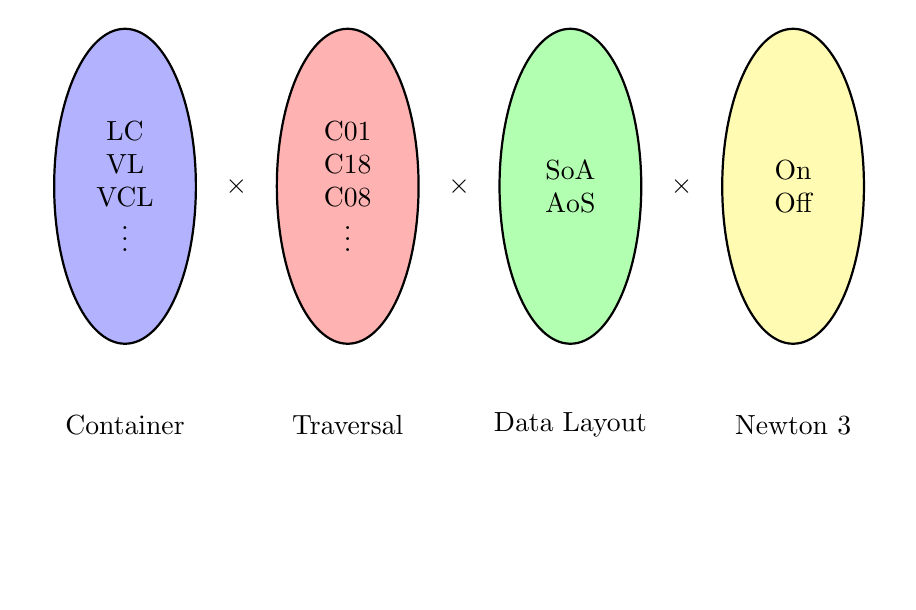
\begin{tikzpicture}[
                node distance=1cm,
                thick,
                every node/.style={
                        draw,
                        ellipse,
                        minimum width=1.8cm,
                        minimum height=4cm,
                        align=center
                    },
                textnode/.style={
                        draw=none,
                        align=center
                    }
            ]

            % Nodes with colors
            \node[fill=blue!30] (A) {LC\\VL\\VCL\\ \vdots};
            \node[fill=red!30, right=of A] (B) {C01\\C18\\C08\\ \vdots};
            \node[fill=green!30, right=of B] (C) {SoA\\AoS};
            \node[fill=yellow!30, right=of C] (D) {On\\Off};

            % Text underneath ellipses with matching colors
            \node[textnode, below=-1cm of A, ] (Atext) {Container};
            \node[textnode, below=-1cm of B, ] (Btext) {Traversal};
            \node[textnode, below=-1cm of C, ] (Ctext) {Data Layout};
            \node[textnode, below=-1cm of D, ] (Dtext) {Newton 3};

            % Crosses between the nodes
            \draw[->, draw=none] (A) -- (B) node[midway, draw=none] {$\times$};
            \draw[->, draw=none] (B) -- (C) node[midway, draw=none] {$\times$};
            \draw[->, draw=none] (C) -- (D) node[midway, draw=none] {$\times$};

        \end{tikzpicture}
    \end{center}


\end{frame}



\begin{frame}{Traditional MD Engines}


    \begin{textblock*}{3.5cm}(8.5cm,2.2cm)
        \includegraphics[width=3.5cm]{figures/gromacs-logo.png}
    \end{textblock*}
    \begin{textblock*}{3.5cm}(8.5cm,4cm)
        \includegraphics[width=3.5cm]{figures/lammps-logo.png}
    \end{textblock*}
    \begin{textblock*}{3cm}(8.5cm,5.3cm)
        \begin{center}

            \includegraphics[width=1.5cm]{figures/ls1-logo.png}
        \end{center}
    \end{textblock*}


    \begin{itemize}
        \item Based on a single container type
              \begin{itemize}
                  \item GROMACS: Verlet Cluster List
                  \item LAMMPS: Verlet List
                  \item ls1 mardyn: Linked Cells
              \end{itemize}
        \item Performance through:
              \begin{itemize}
                  \item Hardware aware SIMD vectorization
                  \item Memory layout optimization
                  \item Manual tuning to target hardware
              \end{itemize}
        \item Drawbacks:
              \begin{itemize}
                  \item Suboptimal for some scenarios / states
                  \item Manual tuning effort
              \end{itemize}
    \end{itemize}

\end{frame}

\section{AutoPas Framework}

\begin{frame}
    \frametitle{What is AutoPas?}

    \begin{textblock*}{5cm}(9cm,1.8cm)
        \includegraphics[width=3cm]{figures/AutoPasLogo}
    \end{textblock*}

    \begin{itemize}
        \item Library for arbitrary N-body simulations
        \item Implements all algorithms
        \item Idea: Switch between algorithms
              \begin{itemize}
                  \item[$\rightarrow$] Guarantee optimal performance
              \end{itemize}

        \item Tuning Strategies:
              \begin{itemize}
                  \item Find optimal configuration
                  \item Different strategies available
              \end{itemize}
    \end{itemize}

    \begin{textblock*}{4cm}(8.2cm,3cm)
        \begin{figure}
            \includegraphics[width=4cm]{figures/AutoPasLibraryStructure.png}
            \caption{ \scriptsize{\cite{Newcome2023Poster}}}

        \end{figure}
    \end{textblock*}

\end{frame}



\section{Auto-Tuning in AutoPas}

\begin{frame}
    \frametitle{Auto-Tuning in AutoPas}

    \begin{itemize}
        \item Divide simulation into Tuning- and Simulation-Phase
        \item Tuning-Phase:
              \begin{itemize}
                  \item Tuning Strategies suggest configurations
                  \item Measure promising configurations
                  \item Choose best configuration
              \end{itemize}
    \end{itemize}

    \begin{center}
        \includegraphics[width=1\textwidth]{figures/timing.png}
    \end{center}
\end{frame}

\begin{frame}
    \frametitle{Tuning Strategies}

    \begin{center}

        {\footnotesize

            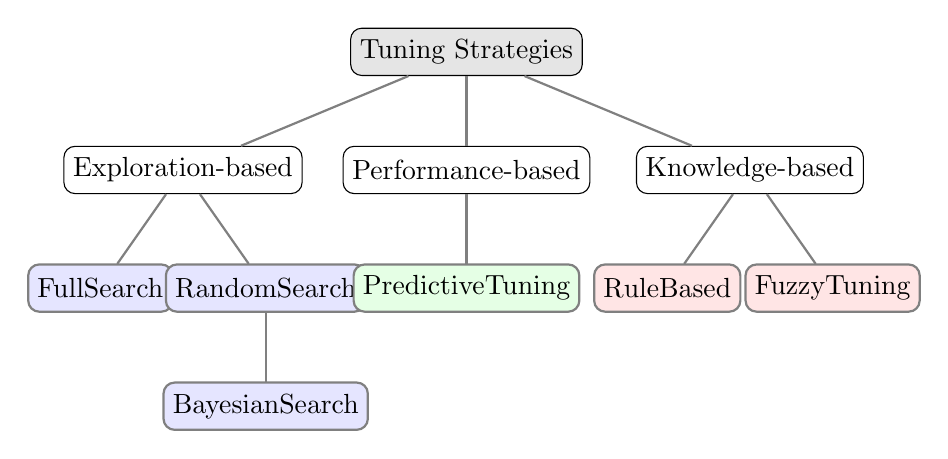
\begin{tikzpicture}[
                    level distance=1.5cm,
                    level 1/.style={sibling distance=3.6cm},
                    level 2/.style={sibling distance=2.1cm},
                    every node/.style={align=center, rounded corners, draw, fill=white, minimum height=0.6cm},
                    edge from parent/.style={thick, draw=gray}
                ]
                \node[fill=gray!20]{Tuning Strategies}
                child{
                        node[]{Exploration-based}
                        child{node[fill=blue!10]{FullSearch}}
                        child{node[fill=blue!10]{RandomSearch}
                                child{node[fill=blue!10]{BayesianSearch}}
                            }
                    }
                child{
                        node[]{Performance-based}
                        child{node[fill=green!10]{PredictiveTuning}}
                    }
                child{
                        node[]{Knowledge-based}
                        child{node[fill=red!10]{RuleBased}}
                        child{node[fill=red!10]{FuzzyTuning}}
                    };
            \end{tikzpicture}

        }
    \end{center}

\end{frame}

\begin{frame}{Benefits of Auto-Tuning}
    \begin{itemize}
        \item Optimal configuration
              \begin{itemize}
                  \item for every scenario
                  \item for every hardware
                  \item throughout the simulation
              \end{itemize}
        \item Shown to improve performance in various scenarios
        \item No manual tuning effort
        \item AutoPas: Optimal Black-Box for N-body simulations
    \end{itemize}
\end{frame}

\begin{frame}{Problems of Auto-Tuning}
    \begin{itemize}
        \item Overhead from evaluating suboptimal configurations
              \begin{itemize}
                  \item Orders of magnitude slower!
              \end{itemize}
        \item Unnecessary periodic re-tuning
    \end{itemize}
    \begin{center}
        \includegraphics[width=0.82\textwidth]{figures/unnecessary-tuning-phases.png}
    \end{center}
\end{frame}



\section{Early Stopping Optimization}


\begin{frame}{Early Stopping Idea}

    \begin{itemize}
        \item Each configuration gets evaluated multiple times
        \item Optimization: Abort resampling early if performance is poor
        \item Two possible strategies:
              \begin{itemize}
                  \item Stop after first poor sample
                  \item Stop during evaluation
              \end{itemize}
    \end{itemize}

    \vspace{0.8cm}

    \begin{center}
        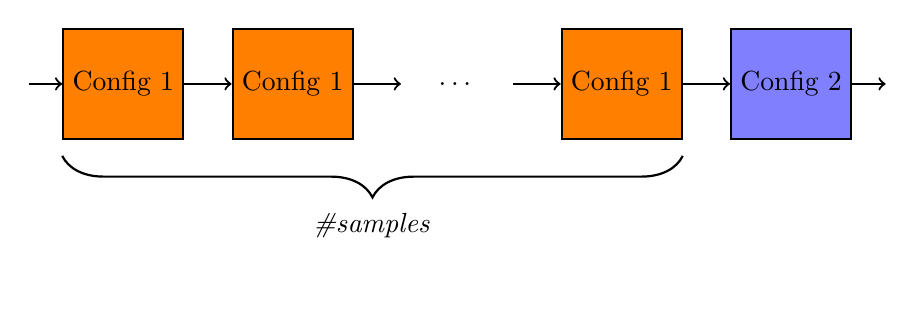
\begin{tikzpicture}[
                node distance=1.2cm and 0.6cm,
                every node/.style={draw, minimum width=1.4cm, minimum height=1.4cm, align=center},
                thick
            ]

            % Define nodes
            \node[fill=orange] (box1) {Config 1};
            \node[right=of box1,fill=orange] (box2) {Config 1};
            \node[right=of box2, style={draw=none}] (box3) {$\dots$};
            \node[right=of box3,fill=orange] (dots) {Config 1};
            \node[right=of dots,fill=blue!50] (boxN) {Config 2};

            % Arrows connecting boxes
            \draw[thick,<-] (box1) -- ++(-1.2,0);
            \draw[thick,->] (box1) -- (box2);
            \draw[thick,->] (box2) -- (box3);
            \draw[thick,->] (box3) -- (dots);
            \draw[thick,->] (dots) -- (boxN);
            \draw[thick,->] (boxN) -- ++(1.2,0);

            % Curly brace underneath the boxes
            \draw[decorate, decoration={brace, amplitude=15pt, mirror}, thick]
            ($(box1.south west) + (0,-0.2)$) -- ($(dots.south east) + (0,-0.2)$)
            node[midway, below=5pt,draw=none] {\textit{\#samples}};



        \end{tikzpicture}
    \end{center}
\end{frame}


\begin{frame}
    \frametitle{Naive Early Stopping}

    \begin{itemize}
        \item Changes to AutoPas are minimal
              \begin{itemize}
                  \item Keep track of best performance seen so far
                  \item $slowdownFactor = \frac{t_{\text{sample}}}{t_{\text{best}}}$
                  \item Call \texttt{retune()} if $slowdownFactor$ exceeds threshold
              \end{itemize}


        \item Hyperparameter: $allowedSlowdownFactor$

        \item Which $allowedSlowdownFactor$ should be used?
              \begin{itemize}
                  \item $allowedSlowdownFactor \rightarrow 1$: Many spurious aborts
                  \item $allowedSlowdownFactor \rightarrow \infty$: No early stopping
              \end{itemize}
    \end{itemize}
\end{frame}

\begin{frame}{Benchmark: Exploding Liquid + PredictiveTuning}

    \begin{itemize}
        \item Optimal at $allowedSlowdownFactor = 5$
        \item From 28.6s to 23.2s
              \begin{itemize}
                  \item[$\rightarrow$] 18.9\% reduction
              \end{itemize}
    \end{itemize}


    \begin{figure}[H]
        \centering

        \includegraphics[width=0.92\columnwidth]{../../data/explodingLiquid/cluster/predictiveTuning/analytics/total_time_average_full_scale.png}


    \end{figure}

\end{frame}


\begin{frame}{Early Stopping Insights}

    \begin{itemize}
        \item Should be combined with good tuning strategy
        \item Never increased simulation time
        \item $allowedSlowdownFactor$ probably not universal
        \item Future work needed
              \begin{itemize}
                  \item More benchmarks
                  \item Improved early stopping mechanism
                  \item Investigate other stopping criteria
              \end{itemize}
    \end{itemize}
\end{frame}


\begin{frame}{Summary}
    \begin{itemize}
        \item Many algorithmic choices in MD simulations
              \begin{itemize}
                  \item No silver bullet!
              \end{itemize}
        \item AutoPas: Optimal Black-Box for N-body simulations
              \begin{itemize}
                  \item Auto-Tuning very beneficial
                  \item But: Overhead from tuning
              \end{itemize}
        \item Early Stopping Optimization
              \begin{itemize}
                  \item Minimal changes to AutoPas
                  \item Promising improvements
              \end{itemize}
    \end{itemize}
\end{frame}



\begin{frame}
    \begin{center}
        \vspace{1cm}
        {\large \textbf{Thank you for your attention!}}

        \vspace{2cm}

        \Huge{Questions?}
    \end{center}
\end{frame}




\begin{frame}[allowframebreaks, noframenumbering]
    \frametitle{References}
    \footnotesize
    \bibliographystyle{apalike}
    \bibliography{literature}
\end{frame}

\appendix




\end{document}